\documentclass[
oneside,
a4paper,
12pt,
titlepage]
{article}
\usepackage[english]{babel}

% \usepackage[LANGUAGE]{babel} % must be set in a per-file manner
\usepackage[utf8]{inputenc}
\usepackage{graphicx} % notwendig für das Einbetten von Bildern s. http://en.wikibooks.org/wiki/LaTeX/Importing_Graphics
%\usepackage{float} % s. http://tex.stackexchange.com/questions/119799/text-next-to-image
\usepackage{amsmath}
\usepackage{amssymb}
\usepackage{fontspec}
\usepackage{unicode-math}
\usepackage{caption}
\usepackage{geometry}
\usepackage{booktabs}
\usepackage{tabularx} % notwendig für Zeilenumbruch in Tabellenzelle http://tex.stackexchange.com/questions/2441/how-to-add-a-forced-line-break-inside-a-table-cell
\usepackage{longtable}
\usepackage{tabu}
\usepackage{multirow}
%\usepackage{fixltx2e} % ermöglicht \textsubscript; verträgt sich nicht mit der [H]-Option von float-Umgebungen
\usepackage{amsthm}
\usepackage{floatrow} % verträgt sich nicht mit float
\usepackage{calc}
\usepackage{setspace} % notwendig zur Festsetzung des Zeilenabstands http://tex.stackexchange.com/questions/74496/how-to-use-times-roman-nimbus-roman-with-fontspec-under-linux-and-lualatex
\usepackage{siunitx} % notwendig für Einheiten in textmode s. http://tex.stackexchange.com/questions/9043/should-greek-letters-inserted-in-text-using-math-mode-mostly-always-be-italic
\usepackage{tikz} % Ermöglicht das Erstellen von Grafiken in LaTeX
\usepackage{circuitikz} % create circuitry
\usepackage{chngcntr} % Ermöglicht das Umschalten von Zählern
\usepackage{paralist} % s.S. 136 Companion
\usepackage{enumitem} % `enumitem´ and `paralist´ seem to conflict
\usepackage{fancyhdr} % aus PFA_woerterbuch.tex
\usepackage{csquotes} % ermöglicht die Verwendung sprachspezifischer Anführungszeichen durch biblatex
\usepackage{textcomp} % um in textmode Minuszeichen schreiben zu können s. http://tex.stackexchange.com/questions/24423/writing-a-negative-number-in-text-mode-9-or-9
\usepackage{upgreek}
\PassOptionsToPackage{hyphens}{url}
\usepackage{hyperref}
\usepackage[sort]{cleveref}
% \PassOptionsToPackage{hyphens}{url}\usepackage[colorlinks=false]{hyperref} % s.S. 50 biblatex-Dokumentation und http://tex.stackexchange.com/questions/3033/forcing-linebreaks-in-url
% \usepackage{url} % probably not necessary, since `url´ is loaded by `hyperref´
\usepackage{commath}
\usepackage{pdflscape}
\usepackage{listings}  %% For inserting and syntax highlighting source code files.
%% \usepackage{minted}  %% For inserting and syntax highlighting source code files.
\usepackage{tracklang}  %% Required by package "datetime2".
\usepackage{datetime2}  %% For inserting dates and times in different formats.
\usepackage{interval}

%%% Local Variables:
%%% mode: latex
%%% TeX-master: "../MasArThesis.tex"
%%% End:

% This file contains both package specific and LaTeX-internal settings;
% `package specific´ means every setting related to the respective package, even if the setting is done via LaTeX primitives (e.g., `\setcounter´)
% `LaTeX-internal´ means only those settings, which cannot be attributed to a specific package;
% CONVENTIONS:
% -comments ought to be placed on the line on which the command/option they refer to ends 
% -when several options are given in one pair of brackets/curly braces, each one should be separated by a newline character, including the first option)

%%%%%%%%%%%%%%
%% interval %%
%%%%%%%%%%%%%%
\intervalconfig{soft open fences}

%%%%%%%%%%%%%%
%% geometry %%
%%%%%%%%%%%%%%
\geometry{
  % margin=2.5cm % for one-sided documents (this requires `\documentclass[oneside…´)
  margin=2cm,
  inner=3cm,
  % inner=2.5cm, % for two-sided documents (this requires `\documentclass[twoside…´)
  % outer=3.5cm, % for two-sided documents (this requires `\documentclass[twoside…´)
  a4paper
}

%%%%%%%%%%%%%
%% caption %%
%%%%%%%%%%%%%
\captionsetup{
  font=footnotesize,
  labelfont=bf,
  singlelinecheck=false,
  justification=justified}
  % justification=centering}

%%%%%%%%%%%%%%
%% hyperref %%
%%%%%%%%%%%%%%
\hypersetup{
  colorlinks=false,
  % colorlinks=true,
  linktoc=all}

%%%%%%%%%%%%%%
%% listings %%
%%%%%%%%%%%%%%
\lstset{
  basicstyle=\ttfamily,
  keywordstyle=,
  showstringspaces=false}

%%%%%%%%%%%%%%
%% setspace %%
%%%%%%%%%%%%%%
% \singlespacing
\onehalfspacing
% \doublespacing

%%%%%%%%%%%%%%
%% enumitem %%
%%%%%%%%%%%%%%
\setlist[itemize]{
  topsep=0cm,
  partopsep=0cm,
  itemsep=0cm} % s. p. 9 enumitem

%%%%%%%%%%%%%%
%% tabularx %%
%%%%%%%%%%%%%%
\newcolumntype{C}{>{\centering\arraybackslash}X}
\newcolumntype{L}{>{\raggedright\arraybackslash}X}
\newcolumntype{R}{>{\raggedleft\arraybackslash}X}

%%%%%%%%%%%%%%
%% paralist %%
%%%%%%%%%%%%%%
\setdefaultitem{\textendash}{\textbullet}{$\square$}{}

%%%%%%%%%%%%%%
%% fontspec %%
%%%%%%%%%%%%%%
% \setmainfont{TeX Gyre Termes}
\setmainfont{XITS}

%%%%%%%%%%%%%%%%%%
%% unicode-math %%
%%%%%%%%%%%%%%%%%%
\setmathfont[
math-style=ISO,
bold-style=literal,
% vargreek-shape=TeX  %% Obsolote as of v0.8d (see https://ctan.org/ctan-ann/id/mailman.2585.1485610970.17497.ctan-ann@ctan.org)
]{XITS Math}

%%%%%%%%%%%%%%
%% floatrow %%
%%%%%%%%%%%%%%
\floatsetup[table]{
  style={plaintop},
  font={normalsize}}
  % font={scriptsize}} %% this setting for some reason affected the longtabu environment, but not the tabu environment
\floatsetup[figure]{capposition=bottom}
\newfloatcommand{myffigbox}{figure}[][\myimagewidth]
\newfloatcommand{mykarte}{figure}[][\textwidth]

%%%%%%%%%%%%%
%% siunitx %%
%%%%%%%%%%%%%
\sisetup{
  locale = US, % manages the locale specific display of numbers, SI units, etc.
  % locale = DE,
  list-final-separator = {, and },
  exponent-product = \cdot,
  redefine-symbols = false, % s. p. 62 siunitx
  group-minimum-digits = 3,
  group-digits = integer,
  table-text-alignment = center,
  table-number-alignment = center
}

%%%%%%%%%%%%%%%
%% longtable %%
%%%%%%%%%%%%%%%
\setcounter{LTchunksize}{10}

%%%%%%%%%%%%%%%%%%%%%%%%%%%%%%%%
%% LaTeX: lengths, skips, etc %%
%%%%%%%%%%%%%%%%%%%%%%%%%%%%%%%%
\setlength{\parindent}{0 cm} % indentation of paragraphs
\setlength{\parskip}{10 pt} % extra vertical space between paragraphs; s. p. 2 “Formatvorlage-Waldökosystemmanagement.doc”: “Nach”
\newlength{\myabovetop}
\setlength{\myabovetop}{2\baselineskip}
\newlength{\myimagewidth}
\setlength{\myimagewidth}{5.65cm}
\newlength{\capskip}
\setlength{\capskip}{-0.35cm}
\setlength{\abovecaptionskip}{0.5\baselineskip}
\setlength{\belowcaptionskip}{0.5\baselineskip}

%%%%%%%%%%%%%%%%%%%%%%%%%
%% LaTeX: environments %%
%%%%%%%%%%%%%%%%%%%%%%%%%
\newenvironment{mytable}[2]{\begin{table}[htb]\scriptsize\caption{#1\vspace{\capskip}}\label{#2}}{\end{table}\par} % \vspace notwendig wegen floatrow

%%%%%%%%%%%%%%%%%%%%%
%% LaTeX: counters %%
%%%%%%%%%%%%%%%%%%%%%
\setcounter{topnumber}{2} % s. p. 284 ff. Companion
\setcounter{bottomnumber}{1} % s. p. 284 ff. Companion
\setcounter{totalnumber}{3} % s. p. 284 ff. Companion
\setcounter{figure}{0}

%%% Local Variables:
%%% mode: latex
%%% TeX-master: "../MasArThesis.tex"
%%% End:

% This file contains settings intended for use with documentclass `article´.

%%%%%%%%%%%%%%
%% chngcntr %%
%%%%%%%%%%%%%%
\counterwithout{figure}{section} % counter `figure´ is not reset at the beginning of a new `section´

%%%%%%%%%%%%%%
%% fancyhdr %%
%%%%%%%%%%%%%%
\pagestyle{fancy}
\fancyhead{}
\fancyfoot{}
\fancypagestyle{toc}{ % http://texblog.org/2013/09/16/multiple-page-styles-with-fancyhdr/
\fancyhead{}
\fancyhead[L]{\fontsize{12pt}{1\baselineskip} \selectfont \leftmark \\}
% \fancyhead[R]{\fontsize{10pt}{1\baselineskip} \thepage \\}
\fancyfoot{}
\renewcommand{\footrulewidth}{0.4pt}
\fancyfoot[C]{\fontsize{10pt}{1\baselineskip} \thepage \\}
}
\fancypagestyle{abbrevs_symbols}{ % http://texblog.org/2013/09/16/multiple-page-styles-with-fancyhdr/
\fancyhead{}
\fancyhead[L]{\fontsize{12pt}{1\baselineskip} \selectfont \leftmark \\}
% \fancyhead[R]{\fontsize{10pt}{1\baselineskip} \thepage \\}
\fancyfoot{}
\renewcommand{\footrulewidth}{0.4pt}
\fancyfoot[C]{\fontsize{10pt}{1\baselineskip} \thepage \\}
}
\fancypagestyle{standard}{ % http://texblog.org/2013/09/16/multiple-page-styles-with-fancyhdr/
\fancyhead{}
% \fancyhead[L]{\fontsize{12pt}{1\baselineskip} \selectfont \leftmark \\}
\fancyhead[L]{\fontsize{12pt}{1\baselineskip} \selectfont \firstmark \\}
% \fancyhead[R]{\fontsize{10pt}{1\baselineskip} \thepage \\}
\fancyfoot{}
\renewcommand{\footrulewidth}{0.4pt}
\fancyfoot[C]{\fontsize{10pt}{1\baselineskip} \thepage \\}
}
\fancypagestyle{bibliography}{ % http://texblog.org/2013/09/16/multiple-page-styles-with-fancyhdr/
\fancyhead{}
\fancyhead[L]{\fontsize{12pt}{1\baselineskip} \selectfont \leftmark \\}
% \fancyhead[R]{\fontsize{10pt}{1\baselineskip} \thepage \\}
\fancyfoot{}
\renewcommand{\footrulewidth}{0.4pt}
\fancyfoot[C]{\fontsize{10pt}{1\baselineskip} \thepage \\}
}
\renewcommand{\sectionmark}[1]{%
  \markboth{#1}{}} % s. p. 9 f. fancyhdr
\renewcommand{\subsectionmark}[1]{%
} % to suppress printing of subsection titles in headers (s. `\firstmark´ above)

%%%%%%%%%%%%%%%%%%%%%
%% LaTeX: commands %%
%%%%%%%%%%%%%%%%%%%%%
\renewcommand\topfraction{1.0} % s. p. 284 ff. Companion
\renewcommand\bottomfraction{1.0} % s. p. 284 ff. Companion
\renewcommand\textfraction{0.0} % s. p. 284 ff. Companion 
\renewcommand\floatpagefraction{0.75} % s. p. 284 ff. Companion 
\makeatletter
\renewcommand{\thefigure}{\arabic{figure}}
\renewcommand{\thetable}{\arabic{table}}
\makeatother
\makeatletter
\renewcommand\section{\@startsection
  {section}{1}{0 mm}
  {\myabovetop}
  {0.25\baselineskip}
  {\normalfont\normalsize\bfseries}}
\renewcommand\subsection{\@startsection
  {subsection}{2}{0 mm}
  {\myabovetop}
  {0.25\baselineskip}
  {\normalfont\normalsize\itshape}}
\renewcommand\subsubsection{\@startsection
  {subsubsection}{2}{0 mm}
  {0 pt}
  {0.05\baselineskip}
  {\normalfont\normalsize}}
\makeatother

%%% Local Variables:
%%% mode: latex
%%% TeX-master: "../MasArThesis.tex"
%%% End:

\usepackage[
backend=biber,
% bibstyle=/home/renke/Uni/Formatvorlagen/LaTeX/BibstylePapers,
bibstyle=authoryear,
% citestyle=/home/renke/Uni/Formatvorlagen/LaTeX/CitestylePapers,
citestyle=authoryear-comp,
natbib=false,
mcite=false,
sorting=nyt,
sortcase=false,
sortcites=true,
maxbibnames=99,
maxcitenames=2,
maxitems=2,
uniquename=false,
autocite=plain,
language=autobib,
hyperref=true,
urldate=long,
dateabbrev=false,
date=year,  % cp. https://tex.stackexchange.com/questions/55780/disable-month-in-biblatex-bibliography
giveninits=true,
bibencoding=utf8 % s. p. 42 ff. biblatex
]{biblatex} % s. p. 45 ff. biblatex

% \addbibresource[location=local]{../../Literatur/MODULNAME} % s. p. 71 f. biblatex; must be set in a per-file manner

\renewcommand*{\nameyeardelim}{\space} % http://tex.stackexchange.com/questions/134063/how-to-add-a-comma-between-author-and-year
\renewcommand*{\revsdnamepunct}{\space}
\renewcommand*{\finentrypunct}{}
\renewcommand*\finalnamedelim{%
  \ifnumgreater{\value{liststop}}{2}{\addspace\bibstring{and}\addspace}%
  {\addspace\biband\addspace}}% http://tex.stackexchange.com/questions/67621/biblatex-have-and-in-the-citation-but-in-the-bibliography

\renewbibmacro*{doi+eprint+url}{%  https://tex.stackexchange.com/questions/154864/biblatex-use-doi-only-if-there-is-no-url
\iftoggle{bbx:url} {\iffieldundef{doi}{\usebibmacro{url+urldate}}{}} {}%
\newunit\newblock \iftoggle{bbx:eprint} {\usebibmacro{eprint}} {}%
\newunit\newblock \iftoggle{bbx:doi} {\printfield{doi}} {}}

\DeclareNameAlias{sortname}{last-first} % http://tex.stackexchange.com/questions/12806/guidelines-for-customizing-biblatex-styles/13076#13076

\DeclareNosort{} % http://tex.stackexchange.com/questions/171492/biblatex-biber-is-incorrectly-sorting-entries-with-hyphens-in-their-respective-a
\DeclareNoinit{
  \noinit{\regexp{[\x{2bf}\x{2018}]}}} % http://tex.stackexchange.com/questions/171492/biblatex-biber-is-incorrectly-sorting-entries-with-hyphens-in-their-respective-a

\newcommand{\biband}{\ifcurrentname{labelname}{\addspace \& \addspace}{\addspace \addcomma \addspace}} % http://tex.stackexchange.com/questions/67621/biblatex-have-and-in-the-citation-but-in-the-bibliography

%%% Local Variables:
%%% mode: latex
%%% TeX-master: "../MasArThesis.tex"
%%% End:

\hyphenation{li-mi-ting}
\hyphenation{sev-er-al}
\hyphenation{ag-ri-cul-tur-al}

%%% Local Variables:
%%% mode: latex
%%% TeX-master: "../MasArThesis.tex"
%%% End:

\hyphenation{zu-zu-schrei-ben}
\hyphenation{Ge-bie-te}
\hyphenation{Wunsch-er-fül-lung}
\hyphenation{der-ar-ti-ge}
\hyphenation{be-stim-mten}
\hyphenation{be-stim-mte}
\hyphenation{mo-ra-li-sche}
\hyphenation{mo-ra-li-schem}
\hyphenation{mo-ra-li-schen}
\hyphenation{mo-ra-li-scher}
\hyphenation{mo-ra-li-sches}
\hyphenation{Un-rechts-er-eig-nis}
\hyphenation{Rechts-an-sprü-chen}
\hyphenation{Rechts-an-sprü-che}
\hyphenation{Rechts-an-spruch}
\hyphenation{re-le-vant}
\hyphenation{Re-le-vanz}
\hyphenation{Rah-men-be-ding-ung-en}
\hyphenation{fort-ge-setz-ten}
\hyphenation{fort-ge-setzt}
\hyphenation{Ein-tref-fen}
\hyphenation{Ein-tref-fens}
\hyphenation{Le-bens-chan-cen}
\hyphenation{Le-bens-chan-ce}
\hyphenation{mensch-lich-es}
\hyphenation{mensch-lich}
\hyphenation{mensch-lich-er}
\hyphenation{mensch-lich-en}
\hyphenation{Be-schrän-kung}
\hyphenation{Täu-schung}
\hyphenation{be-tref-fen}
\hyphenation{stell-ver-tre-tend}
\hyphenation{Ge-rech-tig-keits-an-sprüche}
\hyphenation{Un-rechts-zu-stand}
\hyphenation{zwi-schen}
\hyphenation{Pflich-ten}
\hyphenation{un-glei-chen}
\hyphenation{mei-nen}
\hyphenation{Eigen-tums-rechts}
\hyphenation{Eigen-tums-recht}
\hyphenation{Rech-ten}
\hyphenation{zu-sätz-li-cher}
\hyphenation{schlech-ten}
\hyphenation{Nicht-i-den-ti-täts-pro-blem}
\hyphenation{Pro-blem}
\hyphenation{zu-kunfts-o-ri-en-tiert}
\hyphenation{be-sei-ti-gen-den}
\hyphenation{Ei-gen-tums-rech-ten}
\hyphenation{Fa-kul-tät}
\hyphenation{For-schungs-an-stal-ten}
\hyphenation{Mo-del-lie-rung}
\hyphenation{Ver-suchs-an-stalt}
\hyphenation{Durch-mes-ser}
\hyphenation{er-trags-kund-licher}
\hyphenation{grund-flä-chen-ge-steu-er-ten}

%%% Local Variables:
%%% mode: latex
%%% TeX-master: "../MasArThesis.tex"
%%% End:


%% Input settings files specific to this document.
\input{TikZSettings.tex}

\addbibresource[location=local]{../../Literature/MasAr_Literature.bib} % s. S. 71 f. biblatex-Dokumentation

%% AUCTeX style file: ./style/MasArThesis.el

%% Define custom SI units.
\DeclareSIUnit\year{a}

%% Define custom commands (in alphabetical order of command name). Note: macro names may not contain non-letters.
\newcommand{\Beech}[0]{European beech (\emph{Fagus sylvatica} L.)}
\DeclareMathOperator{\diag}{diag}
\newcommand{\loglikelihood}{\ell}
\newcommand{\logNlogDcurve}{log(\(N\))-log(\(D\))-curve}
\newcommand{\NWFVA}{Northwest German Forest Research Institute}
\newcommand{\Ponderosa}[0]{Ponderosa pine (\emph{Pinus ponderosa} \textsc{Douglas})}
\newcommand{\RefEq}[1]{equation~(\ref{#1})}
\newcommand{\RefTab}[1]{Table~\ref{#1}}
\newcommand{\RefFig}[1]{Figure~\ref{#1}}
\newcommand{\SeePage}[1]{(see page \pageref{#1})}
\newcommand{\SeeSection}[1]{(see section \ref{#1})}
\DeclareMathOperator{\sign}{sign}
\newcommand{\SIWrittenTerm}{absolute productivity index of stand}
\newcommand{\Spruce}[0]{Norway spruce (\emph{Picea abies} (L.) H.\textsc{Karst})}
\newcommand{\TopHeight}[0]{h_{100}}
\DeclareMathOperator{\tr}{tr}

\begin{document}

\begin{titlepage}

\begin{center}

\vspace*{5cm}

{\LARGE Modeling maximum basal area of pure beech and spruce stands in northwestern Germany \\}

\vspace{2cm}

{\large Author: \\ Renke Christian von Seggern \par}

\vspace{2cm}

{\normalsize Master’s Thesis at the \\
  Faculty of Forest Sciences and Forest Ecology, \\
  Georg-August-Universität Göttingen}

\vspace{0.5cm}

{\normalsize Date of submission: \\ December 20, 2017 \par}

\vspace{0.5cm}

{\normalsize Supervisors: \\ Prof. Dr. Winfried Kurth \\ Prof. Dr. Jürgen Nagel \par}

\end{center}

\end{titlepage}

%%% Local Variables:
%%% mode: latex
%%% TeX-master: "MasArThesis.tex"
%%% End:

\newpage

\input{ToC.tex}
\newpage

\pagestyle{abbrevs_symbols}

{
  \renewcommand{\MakeUppercase}[1]{#1} % http://tex.stackexchange.com/questions/179966/fancyhdr-chaptermark-and-table-of-contents

  \newcommand{\mysectiontitle}{Table of abbreviations and symbols} % set section title as a custom macro to ease mutlitple usage (necessary when using a starred sectioning macro)
  
  \section*{\mysectiontitle{}}
  \label{sec:AbbrevsSymbolsTable}
  
  \markboth{\mysectiontitle{}}{} % http://tex.stackexchange.com/questions/89914/chapter-name-in-the-header-with-chapter
  \addcontentsline{toc}{section}{\mysectiontitle{}} % http://tex.stackexchange.com/questions/35433/creating-unnumbered-chapters-sections-plus-adding-them-to-the-toc-and-or-header
  
  % \begin{table}[H]
  %   \centering
  \begin{longtabu}{l L l}
    \toprule
    Symbol & Description & Unit \\
    \midrule
    \endfirsthead
    Symbol & Description & Unit \\
    \midrule
    \endhead
    \bottomrule
    \endlastfoot
    \(CV(\uplambda)\) & cross validation sum of squares for smoothing parameter \(\uplambda\) \\
    \(D\) & average diameter (by basal area) & \si{\centi\meter} \\
    \(\diag(\symbf{x})\) & diagonal matrix with main diagonal \(\symbf{x}\) \\
    \(\erf\) & error function \\
    \(\exp\) & exponential function \\
    \(\mathbb{E}(x)\) & expectation of variable \(x\) \\
    \(G\) & basal area & \si{\square\meter} \\
    GAM & generalized additive model & \\
    GAMLSS & generalized additive model for location, scale, and shape \\
    GCV & generalized cross validation & \\
    \(GCV(\uplambda)\) & generalized cross validation sum of squares for smoothing parameter \(\uplambda\) \\
    GLM & generalized linear model & \\
    \(\TopHeightMath{}\) & top height, height of dominant trees & \si{\meter} \\
    \(\StandAgeVariableMath{}\) & stand age variable (top height at age \(x\) if the stand were yield class \num{1}) & \si{\meter} \\
    % \(k\) & constant (varying with species) & \\
    \(\loglikelihood(x)\) & log-likelihood of \(x\) \\
    LM & Linear Model & \\
    \(\ln\) & natural logarithm \\
    \(\log\) & decadic logarithm \\
    \(N\) & stand density & \si{\per\hectare} \\
    % \(s\) & slope of the \logNlogDcurve{} \\
    \(\ProductivityIndexMath\) & \ProductivityIndexText{} (\(\TopHeightMath{}\) at age \SI{100}{\year}) & \si{\meter} \\
    SCAM & shape constrained additive model \\
    \(\sign\) & sign function \\
    \(\tr(\symbf{A})\) & trace of square matrix \(\symbf{A}\) \\
    % UBRE & un-biased risk estimator \\
  \end{longtabu}
  % \end{table}
}

%% Reset table counter.
\setcounter{table}{0}

%%% Local Variables:
%%% mode: latex
%%% TeX-master: "MasArThesis.tex"
%%% End:

\newpage

\pagestyle{standard}
\pagenumbering{arabic}

\section{Introduction}

\section{Material and Methods}
\section{Auswahl der Daten}
\subsection{Reineke-Gleichung}
\begin{frame}[c]
  \visible<\theFirstElement->{
    \begin{center}
      \begin{minipage}{0.40\textwidth}
        \centerline{\(\mylog(N) = \textcolor{red}{s} \log(D) + k\)}
        \vspace{\captiondistance}
        \mycaption{Gleichung 1}{Bestandesdichte in Abhängigkeit von mittlerem Durchmesser (Quelle: [1]). \\
          \(N\): Bestandesdichte [\si{\per\hectare}] \\
          \(s\): \textcolor{red}{Steigung} \\
          \(D\): Durchmesser des Grundflächenmittelstammes [\si{\centi\meter}] \\
          \(k\): Konstante (artabhängig)}
      \end{minipage}
    \end{center}

    % \begin{align*}
      % \myscalebox{N} & \myscalebox{: \text{Bestandesdichte [ha\textsuperscript{-1}]}} \\[-3mm]
      % \myscalebox{s} & \myscalebox{: \text{Steigung (}\widehat{=}\text{ \textcolor{red}{Mortalitätsrate})}} \\[-3mm]
      % \myscalebox{D} & \myscalebox{: \text{Durchmesser des Grundflächemittelstammes [cm]}} \\[-3mm]
      % \myscalebox{k} & \myscalebox{: \text{Konstante (artabhängig)}} \\[-3mm]
    % \end{align*}
  }

  \begin{itemize}
  \item<\theSecondElement-> Literatur: \\
    Steigung scheint art- und standortabhängig zu sein (s. z.B. [2])
  \item<\theSecondElement-> Lösungsansatz: \\
    artabhängiger Korridor ,,erlaubter`` Steigungen, begrenzt durch unteren Schwellwert (\(m_u\)) und oberen Schwellwert (\(m_o\))
  \end{itemize}
\end{frame}

\subsection{Auswahlmechanismus}
\begin{frame}[c]
  \begin{columns}
    \begin{column}{0.5\textwidth}
      \visible<\theFirstElement->{
        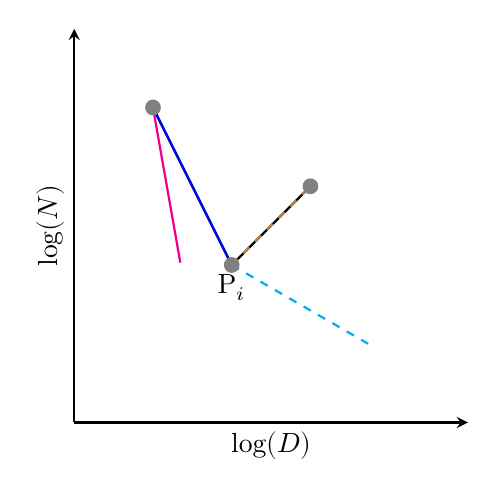
\begin{tikzpicture}[>=stealth]
          %% Coordinate system.
          \draw[black,thick,->] (0,0) -- (5,0);  %% x-axis
          \draw[black,thick,->] (0,0) -- (0,5);  %% y-axis
          \node[anchor=north] at (2.5,0) {\(\log(D)\)};  %% x-axis title
          \node[anchor=south,rotate=90] at (0,2.5) {\(\log(N)\)};  %% y-axis title
          
          %% Specify point coordinates.
          \coordinate (Pi-1) at (1,4);
          \coordinate (Pi) at (2,2);
          \coordinate (Pi+1) at (3,3);

          %% Lines.
          \visible<\theFirstElement-\theSecondElement>{\draw[black,thick] (Pi-1) -- (Pi) -- (Pi+1);}
          \visible<\theSecondElement->{\draw[magenta,thick] (Pi-1) -- ++(280:2cm);}
          \visible<\theSecondElement->{\draw[blue,thick] (Pi-1) -- (Pi);}
          \visible<\theThirdElement->{\draw[cyan,thick,dashed] (Pi) -- ++(330:2cm);}
          \visible<\theThirdElement->{\draw[brown,thick,dashed] (Pi) -- (Pi+1);}

          %% Points.
          \fill[gray] (Pi-1) circle (0.1);
          \fill[gray] (Pi) circle (0.1);
          \fill[gray] (Pi+1) circle (0.1);

          %% Text.
          % \node[anchor=south] at (Pi-1) {\(\text{P}_{i-1}\)};
          \node[anchor=north] at (Pi) {\(\text{P}_i\)};
          % \node[anchor=south] at (Pi+1) {\(\text{P}_{i+1}\)};

        \end{tikzpicture}
        \captionsep{}
        \mycaption{Abbildung 1}{Schematische Darstellung der Funktionsweise des Auswahlmechanismus.}
      }
    \end{column}
    \begin{column}{0.5\textwidth}
      \visible<\theFirstElement->{\(\text{P}_i\) wird ausgewählt, wenn}
      \begin{enumerate}
      \item<\theFirstElement-> es mind. einen benachbarten Punkt gibt (\ding{51}) und
      \item<\theSecondElement-> Steigung \(\textcolor{blue}{s_1} \geq \textcolor{magenta}{m_u}\) (\ding{51}) und
      \item<\theThirdElement-> Steigung \(\textcolor{brown}{s_2} \leq \textcolor{cyan}{m_o}\) (\ding{55}).
      \end{enumerate}
    \end{column}
  \end{columns}
\end{frame}

\subsection{Beispiel: Buche}
\begin{frame}[c]
  \visible<1->{
    \centerline{
      \begin{minipage}{0.9\textwidth}
        \includegraphics[width=1.0\textwidth]{../../Graphics/Presentation/logDlogNPlotsBeforeAfterDataSelectionBeech.pdf}
        \captionsep{}
        \mycaption{Abbildung 2}{Beobachteter Zusammenhang zwischen Bestandesdichte \(N\) und mittlerem Durchmesser \(D\).  Farbige Linien verbinden Beobachtungen eines Bestandes. Gestrichelte bzw. durchgezogene schwarze Linien stellen den oberen bzw. unteren Schwellwert der noch ,,erlaubten`` Steigungen beispielhaft dar. \\
          A: vor Anwendung des Auswahlmechanismus \\
          B: nach Anwendung des Auswahlmechanismus}
      \end{minipage}}}
\end{frame}

%%% Local Variables:
%%% mode: latex
%%% TeX-master: "MasArPresentation.tex"
%%% End:

\subsection{Description of data sets}

The data set size for \Beech{} is reported in \RefTab{tab:ObservationsCountPerEdvidBeech}.  The data set comprises 18 sample plots, with a total of 63 observations and a mean of \num{3.5} observations per sample plot.  The data set size for \Spruce{} is reported in \RefTab{tab:ObservationsCountPerEdvidSpruce}.  The data set comprises 28 sample plots, with a total of 100 observations and a mean of \num{3.6} observations per sample plot.  In both data sets, the number of observations per sample plot ranges from \numrange{2}{8}.

The geographical location and the altitude above sea level of sample plots are reported in \RefFig{fig:LocationsSamplePlots} and \RefFig{fig:SpeciesAltitudeOfSamplePlots}, respectively.  The dots in the plots of both figures do not add up to the total number of sample plots of the respective species because some sample plots were part of the same trial and therefore shared the same geographical location and altitude.  In the \Beech{} data set, altitude above sea level spans \SI{525}{\meter}, ranging from \SIrange{40}{565}{\meter}, with a mean of \SI{313.2}{\meter}.  In the case of \Spruce{} it spans \SI{730}{\meter}, ranging from \SIrange{20}{750}{\meter}, with a mean of \SI{410.5}{\meter}.

In Figures \ref{fig:StandAgeTopHeightYieldClassClassification}, \ref{fig:StandAgeSiteIndexYieldClassClassification}, and \ref{fig:StandAgeBasalAreaYieldClassClassification}, dot color signifies the (fractional) yield class of the respective observation.  Classification of observations into yield classes required multiple steps, which were undertaken separately for each species.  First, for all observations the absolute site index \(SI\) in \si{\meter} was computed using the equation
\begin{equation}
  \label{eq:NagelFunctionSolvedForSI}
  SI = \frac{\TopHeight(x) + 49.872 - 7.3309 \cdot \ln(x) - 0.77338 \cdot \ln(x)^2 }{0.52684 + 0.10542 \cdot \ln(x)} ,
\end{equation}
\parencite{Nagel1999} where \(x\) is stand age and \(\TopHeight(x)\) is top height in \si{\meter} at age \(x\).  Next, a sequence of \(\TopHeight{}\)-values at age \SI{100}{\year} was generated, ranging from yield class \num{4} to yield class \num{-2}, using an increment of \SI{0.1}{\meter}, thus also covering fractional yield classes.  Values for yield classes \numrange{4}{1} were taken from \textcite{Schober1995} for moderately thinned stands of the respective species, while values for yield classes \numrange{0}{-2} were linearly interpolated from those for yield classes \numlist{2; 1}.   This sequence was then restricted to the range between the best yield class needed to include the lowest observed \(SI\) and the worst yield class needed to include the highest observed \(SI\).  A color palette matching this restricted sequence was then generated, ranging from red (worst yield class observed) over yellow and green to blue (best yield class observed).  Each observed \(SI\) was then mapped to the color representing the corresponding \(\TopHeight{}\)-value.  Considering \RefFig{fig:StandAgeTopHeightYieldClassClassification}, the method of yield class classification yielded plausible results in both data sets:  for a given top height, yield class gradually worsens as stand age increases.

As can be seen from \RefFig{fig:StandAgeTopHeightYieldClassClassification}, several differences between the \Beech{} data set and the \Spruce{} data set exist.  In the former, stands are notably older and cover a wider range of ages, with stand age ranging from \SIrange{35}{153.6}{\year} (difference: \SI{118.6}{\year}), whereas in the latter it ranges from \SIrange{15}{113}{\year} (difference: \SI{98}{\year}).  Consequently, stands in the \Beech{} data set have a higher top height, with \(\TopHeight\) ranging from \SIrange{16.3}{39.2}{\meter} (difference: \SI{22.9}{\meter}), but \Spruce{} stands cover a slightly wider range of top heights, with \(\TopHeight{}\) ranging from \SIrange{9.1}{33.3}{\meter} (difference: \SI{24.2}{\meter}).   In the case of \Beech{}, the maximal top height of all observations was reached by a sample plot of intermediate yield class (\(\approx{} 1\)) compared to the other sample plots in the data set.   In the case of \Spruce{}, the maximal top height of all observations was reached by a sample plot of bad yield class (\(\approx{} 2\)) compared to the other sample plots in the data set.

\RefFig{fig:StandAgeSiteIndexYieldClassClassification} shows the observed development of site index \(SI\) over stand age for \Beech{} (top) and \Spruce{} (bottom).  For all sample plots in both data sets, the site index changed at least once during stand development.  However, for several sample plots the direction of this change itself differs during stand development and there does not seem to be a general direction to which site index changes adhered.  The \Beech{} data set covers a narrower range of site indices and consequently yield classes than the \Spruce{} one, with \(SI\) ranging from \SIrange{23.7}{38.3}{\meter} (difference: \SI{14.6}{\meter}) and yield class ranging from \numrange{4}{-1} in the former, whereas for \Spruce{} \(SI\) ranges from \SIrange{24.1}{45.2}{\meter} (difference: \SI{21.1}{\meter}) and yield class from \numrange{4}{-2}.

\RefFig{fig:StandAgeBasalAreaYieldClassClassification} depicts the observed development of basal area \(G\) over stand age for \Beech{} (top) and \Spruce{} (bottom).
The \Beech{} data set has a higher minimal and a lower maximal basal area and covers a narrower range of basal areas compared to the \Spruce{} one, with \(G\) ranging from \SIrange{12.6}{51.3}{\square\meter} (difference: \SI{38.7}{\square\meter}) in the former, and from \SIrange{10.8}{79.8}{\square\meter} (difference: \SI{69}{\square\meter}) in the latter.

\newpage{}  %% TESTING (this is meant only to prevent "misplaced \cr" errors due to the following longtable stretching across page breaks)
\begin{singlespace}
  {\tabulinesep=2mm
    \begin{longtabu}{l l S L}
      \caption{Number of observations per sample plot, total number of sample plots, and total number of observations in the \Beech{} data set. \label{tab:ObservationsCountPerEdvidBeech}} \\
      \toprule
      & Sample plot ID & {Number of observations} &  \\
      \midrule
      \endhead
      \bottomrule
      \endlastfoot
      & 00521004 & 4 \\
      & 04221005 & 5 \\
      & 08021003 & 2 \\
      & 58321003 & 8 \\
      & 8942102A & 4 \\
      & 8942102B & 2 \\
      & 89521002 & 5 \\
      & 89621002 & 4 \\
      & 89721006 & 2 \\
      & 90421001 & 2 \\
      & 99321000 & 4 \\
      & A1321300 & 2 \\
      & A8121011 & 2 \\
      & H1021001 & 2 \\
      & J5121001 & 4 \\
      & J5121005 & 5 \\
      & J5121007 & 4 \\
      & Z72NAT01 & 2 \\
      Total & 18 & 63 \\
      % Mean & & 3.5 \\
      % Median & & 4 \\
    \end{longtabu}
  }
\end{singlespace}

\newpage{}  %% TESTING (this is meant only to prevent "misplaced \cr" errors due to the following longtable stretching across page breaks)
\begin{singlespace}
  {\tabulinesep=2mm
    \begin{longtabu}{l l S L}
      \caption{Number of observations per sample plot, total number of sample plots, and total number of observations in the \Spruce{} data set. \label{tab:ObservationsCountPerEdvidSpruce}} \\
      \toprule
      & Sample plot ID & {Number of observations} &  \\
      \midrule
      \endhead
      \bottomrule
      \endlastfoot
      & 05451102 & 5 \\
      & 06451102 & 5 \\
      & 07151102 & 8 \\
      & 07551103 & 7 \\
      & 07551105 & 3 \\
      & 4665111A & 2 \\
      & 4665112B & 2 \\
      & 4665113B & 2 \\
      & 4665114B & 4 \\
      & 4675112A & 2 \\
      & 4675113A & 3 \\
      & 4675113B & 3 \\
      & 47451104 & 5 \\
      & 55751102 & 3 \\
      & 87021515 & 2 \\
      & 87021517 & 2 \\
      & 87021522 & 2 \\
      & J6351121 & 2 \\
      & J6351141 & 3 \\
      & S1051103 & 3 \\
      & S1751101 & 3 \\
      & S1851101 & 4 \\
      & S1951101 & 3 \\
      & S2051102 & 3 \\
      & S2151101 & 2 \\
      & S2251101 & 5 \\
      & S2451102 & 4 \\
      & S2651104 & 8 \\
      Total & 28 & 100 \\
      % Mean & & 3.6 \\
      % Media & & 3 \\
    \end{longtabu}
  }
\end{singlespace}

\begin{figure}[H]
  \centering
  \includegraphics[width=1.0\textwidth]{../../Graphics/Thesis/LocationsSamplePlots.pdf}
  \caption{Geographical location of the sample plots of \Beech{} (left) and \Spruce{} (right) in Germany.}
  \label{fig:LocationsSamplePlots}
\end{figure}

\begin{figure}[H]
  \centering
  \includegraphics[width=0.5\textwidth]{../../Graphics/Thesis/SpeciesAltitudeOfSamplePlots.pdf}
  \caption{Altitude above sea level of sample plots.}
  \label{fig:SpeciesAltitudeOfSamplePlots}
\end{figure}

\newpage{}
\begin{figure}[H]
  \centering
  \includegraphics[width=1\textwidth]{../../Graphics/Thesis/StandAgeTopHeightYieldClassClassification.pdf}
  \caption{Observed relationship between stand age and top height \(\TopHeight\) for \Beech{} (top) and \Spruce{} (bottom).  Each dot represents one observation.  Lines connect observations belonging to the same sample plot.  The dot color signifies the (fractional) yield class of the respective observation, ranging from red (worst yield class observed) over yellow and green to blue (best yield class observed).  Yield class classification was based on \textcite{Schober1995} (moderately thinned stands).  Note the different yield class ranges in both plots.}
  \label{fig:StandAgeTopHeightYieldClassClassification}
\end{figure}

\newpage{}
\begin{figure}[H]
  \centering
  \includegraphics[width=1\textwidth]{../../Graphics/Thesis/StandAgeSiteIndexYieldClassClassification.pdf}
  \caption{Observed relationship between stand age and site index \(SI\) for \Beech{} (top) and \Spruce{} (bottom).  Each dot represents one observation.  Solid black lines connect observations belonging to the same sample plot.  Dashed lines mark the \(SI\) of yield classes.  Color of dots and dashed lines signifies the (fractional) yield class of the respective \(SI\), ranging from red (worst yield class observed) over yellow and green to blue (best yield class observed). Yield class classification was based on \textcite{Schober1995} (moderately thinned stands).  Note the different yield class ranges in both plots.}
  \label{fig:StandAgeSiteIndexYieldClassClassification}
\end{figure}

\newpage{}
\begin{figure}[H]
  \centering
  \includegraphics[width=1\textwidth]{../../Graphics/Thesis/StandAgeBasalAreaYieldClassClassification.pdf}
  \caption{Observed relationship between stand age and basal area \(G\) for \Beech{} (top) and \Spruce{} (bottom).  Each dot represents one observation.  Lines connect observations belonging to the same sample plot.  The dot color signifies the (fractional) yield class of the respective observation, ranging from red (worst yield class observed) over yellow and green to blue (best yield class observed).  Yield class classification was based on \textcite{Schober1995} (moderately thinned stands).  Note the different yield class ranges in both plots.}
  \label{fig:StandAgeBasalAreaYieldClassClassification}
\end{figure}

% \newpage{}  %% TESTING (this is meant only to prevent "misplaced \cr" errors due to the following longtable stretching across page breaks)
% \begin{singlespace}
  % {\tabulinesep=2mm
    % \begin{longtabu}{L S S}
      % \caption{Summary statistics of the altitude above sea level of the sample plots. \label{tab:AltitudeSummaries}} \\
      % \toprule
      % Statistic & {Beech} & {Spruce} \\
      % \midrule
      % \endhead
      % \bottomrule
      % \endlastfoot
      % Minimum & 40 & 20 \\
      % Mean & 315.6 & 404 \\
      % Median & 363.5 & 445 \\
      % Maximum & 565 & 750 \\
    % \end{longtabu}
  % }
% \end{singlespace}

%%% Local Variables:
%%% mode: latex
%%% TeX-master: "MasArThesis.tex"
%%% End:

\subsection{Model overview}

\RefTab{tab:PresentedModelsOverviewFormulas} provides an overview of the settings used for fitting the models presented in this study.  For each species, 6 different models were fitted: 2 GAMs, one SCAM, and 3 GAMLSSs.  The settings for a given model were the same for \Beech{} and \Spruce{}.  In the case of GAM1 and GAM2, the \texttt{s(\textnormal{\ldots})} formula terms are smooth functions using thin plate regression splines as their function basis.  In the case of SCAM1, the \texttt{s(\textnormal{\ldots}, bs = "micv")} formula term is a smooth function using P-splines constrained to be increasing and concave as its function basis.  In all smooth functions of the GAMS and SCAM, the setting of basis dimension and order of penalty is left to the smooth function.  In the case of GAMLSS1 and GAMLSS2, the \texttt{ps(\textnormal{\ldots})} formula terms are smooth functions using P-splines as their function basis.  In the case of GAMLSS3, the \texttt{pbm(\ldots{})} term is a smooth function using P-splines constrained to be montonone increasing as its function basis.  In all smooth functions of the 3 GAMLSSs, function basis degree was set to 3, function basis order was set to 2, the number of spline knots was set to 20, while selection of the smoothing parameter was left to the smooth function. For all GAMLSSs, the formula reported in \RefTab{tab:PresentedModelsOverviewFormulas} applies only to the location parameter of the assumed probability distribution. All other distribution parameters were modelled as constants (i.e., with formula \texttt{gha \textasciitilde{} 1}).  None of the 6 models assume interaction between the predictor variables.

\begin{table}[H]
  {\tabulinesep=2mm
    \begin{longtabu}{l l l L}
      \caption{Overview of the \texttt{R} functions and formulas used for fitting the models presented in this study. The overview includes
        the model ID,
        the name of the \texttt{R} package (and its version number) which provided the model fitting function,
        the name of the \texttt{R} model fitting function,
        and the formula used in the model fitting function call.
        In the case of GAMLSS1, GAMLSS2, and GAMLSS3, the formula applies only to the location parameter of the assumed probability distribution.
        For all other distribution parameters, the formula was \texttt{gha \textasciitilde{} 1}. \\
        \texttt{gha}: basal area variable \\
        \StandAgeVariableR{}: stand age variable (cp. \RefEq{eq:StandAgeVariable}) \\
        \ProductivityIndexVariableR{}: productivity index variable (cp. \RefEq{eq:SiteClassVariable})
        \label{tab:PresentedModelsOverviewFormulas}} \\
      \toprule
      Model ID & Package (Version) & Fitting function & Formula \\
      \midrule
      \endhead
      \bottomrule
      \endlastfoot
      GAM1 & \texttt{mgcv} (1.8.22) & \texttt{gam} & \texttt{gha \textasciitilde{} s(\StandAgeVariableR{}) + s(\ProductivityIndexVariableR{})} \\
      GAM2 & As above & As above & \texttt{gha \textasciitilde{} s(\StandAgeVariableR{}) + \ProductivityIndexVariableR{}} \\
      SCAM1 & \texttt{scam} (1.2.2) & \texttt{scam} & \texttt{gha \textasciitilde{} s(\StandAgeVariableR{}, bs = "micv") + \ProductivityIndexVariableR{}} \\
      GAMLSS1 & \texttt{gamlss} (5.0.4) & \texttt{gamlss} & \texttt{gha \textasciitilde{} ps(\StandAgeVariableR{}) + ps(\ProductivityIndexVariableR{})} \\
      GAMLSS2 & As above & As above & \texttt{gha \textasciitilde{} ps(\StandAgeVariableR{}) + \ProductivityIndexVariableR{}} \\
      GAMLSS3 & As above & As above & \texttt{gha \textasciitilde{} pbm(\StandAgeVariableR{}) + \ProductivityIndexVariableR{}} \\
      \bottomrule
    \end{longtabu}}
\end{table}

\RefTab{tab:PresentedModelsOverviewDistributions} provides an overview of the probability distributions and link functions employed in the presented models.  Models GAM1, GAM2, and SCAM1 assume basal area to follow Gamma distribution.  The cumulative distribution function of a variable following Gamma distribution is given by
\begin{equation}
  \label{eq:GammaDistributionProbabilityDensityFunction}
  P(X = x|k, \theta) = x^{k - 1} \frac{\exp{\Bigl(\frac{-x}{\theta}\Bigr)}}{\theta^k \upGamma(k)},
\end{equation}
where \(k\) and \(\theta\) are the shape and scale parameter, respectively, and \(\upGamma\) is the Gamma function \parencite{Dormann2013}.  To avoid implausible negative predictions of basal area, the logarithm function was chosen as the link function, rather than the default inverse function.  Models GAMLSS1, GAMLSS2, and GAMLSS3 assume basal area to follow Box-Cox-Cole-Green distribution.  %% CONTINUE HERE with describing the CDF of the BCCG distribution.

\begin{table}[H]
  {\tabulinesep=2mm
    \begin{longtabu}{l l L}
      \caption{Overview of the \texttt{R} distribution functions used for the models presented in this study.  The overview includes
        the model ID,
        the name of the \texttt{R} package (and its version number) which provided the distribution function,
        and the \texttt{R} call of the distribution function used in model fitting.
        \label{tab:PresentedModelsOverviewDistributions}} \\
      \toprule
      Model ID & Package (Version) & Distribution function call \\
      \midrule
      \endhead
      \bottomrule
      \endlastfoot
      GAM1 & \texttt{stats} (3.3.3) & \texttt{Gamma(link = "log")} \\
      GAM2 & As above & As above \\
      SCAM1 & As above & As above \\
      GAMLSS1 & \texttt{gamlss.dist} (5.0.3) & \texttt{BCCGo()} \\
      GAMLSS2 & As above & As above \\
      GAMLSS3 & As above & As above \\
      \bottomrule
    \end{longtabu}}
\end{table}

One main goal in model formulation was to ensure that the fitted models were capable of separating the effects of stand age and productivity index on predicted basal area.  Top height (\(h_{100}\)) was considered an unsuited predictor variable for achieving this goal, since past experience had shown that using this dimension as the predictor variable does not allow identification of a separate productivity index-effect in the model, at least when data set size is rather limited as is the case in the present study.  Therefore, 2 new variables were calculated:  a stand age variable and a productivity index variable, each of which was calculated in such a way as to exclude the effect of the other. The stand age variable was calculated using the equation
\begin{equation}
  \label{eq:StandAgeVariable}
  \StandAgeVariableMath{} = \beta_0 + \beta_1 \cdot \ln(x) + \beta_2 \cdot \ln(x)^2 + \ProductivityIndexYieldClassIMath{} \cdot \bigl(\beta_3 + \beta_4 \cdot \ln(x)\bigr),
\end{equation}
where \(\StandAgeVariableMath{}\) is the top height in \si{\meter} at age \(x\) if the stand were yield class I, \(\ProductivityIndexYieldClassIMath{}\) is the species-specific top height (\(h_{100}\)) at age \SI{100}{\year} of a stand of yield class I and all other terms have the same meaning as in \RefEq{eq:NagelFunctionSolvedForSI} \parencite{Nagel1999}.  The values for \(\ProductivityIndexYieldClassIMath{}\) were taken from \textcite{Schober1995} and are reported in \RefTab{tab:SIYieldClassI}.  By setting \(\ProductivityIndexYieldClassIMath{}\) to a species-specific constant, it was possible to exclude any productivity index-effects from .  Thus, \(h_{100}(x)_{\text{I. YC}}\) only depends on stand age and was therefore chosen as the stand age variable.

\begin{table}[H]
  {\tabulinesep=2mm
    \begin{longtabu}{l S L}
      \caption{Species-specific values of top height (\(h_{100}\)) at age \SI{100}{\year} of a stand of yield class I as reported in \textcite{Schober1995}
        \label{tab:SIYieldClassI}} \\
      \toprule
      Species & {\(\ProductivityIndexYieldClassIMath{}\) [\si{\meter}]} & \\
      \midrule
      \endhead
      \bottomrule
      \endlastfoot
      Beech & 32.4 \\
      Spruce & 35.1 \\
      \bottomrule
    \end{longtabu}}
\end{table}

The productivity index variable was calculated in 2 steps.  First, the \ProductivityIndexText{} was calculated using \RefEq{eq:NagelFunctionSolvedForSI}.  Subsequently, this value was subtracted from the \ProductivityIndexText{} of yield class I using the equation
\begin{equation}
  \label{eq:SiteClassVariable}
  \ProductivityIndexVariableMath{} = SI - \ProductivityIndexYieldClassIMath{},
\end{equation}
where \(\ProductivityIndexVariableMath{}\) is the productivity index variable, \(SI\) has the same meaning as in \RefEq{eq:NagelFunctionSolvedForSI}, and \(\ProductivityIndexYieldClassIMath{}\) has the same meaning as in \RefEq{eq:StandAgeVariable}.  \(\ProductivityIndexVariableMath{}\) is a measure of the performance of a stand relative to a reference stand (here: a stand of yield class I according to \textcite{Schober1995}): high values signify stands which outperform the reference stand, whereas low values indicate low performance stands.  Since both \(SI\) and \(\ProductivityIndexYieldClassIMath{}\) refer to a specific stand age (here: 100 \si{\year}) rather than a variable one, \(\ProductivityIndexVariableMath{}\) is only influenced by stand productivity and not by stand age.  Thus, it is free of any stand age-effects and was therefore chosen as the productivity index variable.

%%% Local Variables:
%%% mode: latex
%%% TeX-master: "MasArThesis.tex"
%%% End:

\subsection{Explanation of GAMs}

Generalized Additive Models (GAMs) are an extension of Generalized Linear Models (GLMs), which in turn build upon Linear Models (LMs).
% In order to explain GAMs, I will therefore first describe LMs and GLMs, before going into detail about GAMs.

% \subsubsection{Distributional assumptions in Linear Models}

A simple LM assumes a metric random variable \(Y\) to linearly depend upon the metric variable \(X\), such that
\begin{equation}
  \label{eq:LinearModel}
  Y = X \beta + \varepsilon
\end{equation}
where \(\beta\) is the coefficient of \(X\) to be estimated and \(\varepsilon_i\) is an independent random variable such that \(\mathbb{E}\bigl(\varepsilon_i\bigr) = 0\) and \(\mathbb{E}\bigl(\varepsilon_i^2\bigr) = \sigma^2\).  To allow testing of hypotheses related to the model described by \RefEq{eq:LinearModel}, additional assumptions about the distribution of \(Y\) and \(\varepsilon\) need to be made.  Specifically, 2 assumptions are made: the residual term \(\varepsilon\) is assumed to follow normal distribution with a mean of zero and a variance of \(\sigma^2\): \(\varepsilon \sim N\bigl(0, \sigma^2\bigr)\); and the response variable \(Y\) is assumed to follow normal distribution with a mean equal to the product of independent variable \(X\) and parameter \(\beta\) and a variance of \(\sigma^2\): \(Y \sim N\bigl(X \beta, \sigma^2\bigr) \) \parencite{Wood2006,Burkschat2012}.

% \subsubsection{Distributional assumptions in Generalized Linear Models}

A GLM has the structure
\begin{equation}
  \label{eq:GeneralizedLinearModel}
  g\bigl(\mu_i\bigr) = \symbf{x}_i \symbf{\beta}~,  %% Command "\symbf" is provided by package "unicode-math" (see unicode-math manual p. 11)
\end{equation}
where \(\mu_i\) is the expectation of response variable \(Y_i\), i.e., \(\mu_i \equiv \mathbb{E}\bigl(Y_i\bigr)\), \(g\) is a smooth monotonic ``link function'', \(\symbf{x}_i\) is the \(i^{\text{th}}\) row of model matrix \(\symbf{X}\), and \(\symbf{\beta}\) is a vector of unknown parameters \parencite{Wood2006,Nelder1972}.
GLMs are an extension of LMs insofar as they also also center around a ``linear predictor'', \(\symbf{X}\symbf{\beta}\), but allow other link functions than the identity function and allow the distribution of the dependent variable to be any distribution from the exponential family, instead of only the normal distribution.  The exponential family consists of distributions whose probability density function can be written as
\begin{equation}
  \label{eq:ExponentialFamilyProbabilityDensityFunction}
  f_{\theta}\bigl(y\bigr) = \exp \bigg( \frac{y \theta - b(\theta)}{a(\Phi)} + c(y, \Phi)\bigg)~,
\end{equation}
where \(a\), \(b\), and \(c\) are arbitrary functions, \(\Phi\) is an arbitrary ``scale'' parameter, and \(\theta\) is the so-called ``canonical parameter'' of the distribution \parencite{Wood2006}.

Building upon GLMs, a GAM has a structure similar to
\begin{equation}
  \label{eq:GeneralizedAdditiveModel}
  g\bigl(\mu_i\bigr) = \symbf{x}_i^* \symbf{\theta} + f_{1}\bigl(x_{1i}\bigr) + f_{2}\bigl(x_{2i}\bigr) + f_{3}\bigl(x_{3i}, x_{4i}\bigr) + \ldots~,
\end{equation}
where \(\mu_i\) again is the expectation of response variable \(Y_i\), i.e., \(\mu_i \equiv \mathbb{E}\bigl(Y_i\bigr)\), the response variable \(Y_i\) follows any exponential family distribution, \(\symbf{x}_i^*\) is a row of the model matrix for any strictly parametric model components, \(\symbf{\theta}\) is the corresponding parameter vector, and the \(f_j\) are smooth functions of the covariates, \(x_k\) \parencite{Wood2006}.  A smooth function may be considered an estimate of the acutal functional relationship between the response variable and the predictor variable to which the smooth function is applied \parencite{Hastie1991}.  Unlike LMs or GLMs, a smooth function is nonparametric, i.e., it does not assume the response variable to follow any specific distribution.
As an explanatory example, consider a model containing one smooth function of one predictor variable with the identity function as the link function,
\begin{equation}
  \label{eq:GeneralizedAdditiveModelSimple}
  y_i = f\bigl(x_i\bigr) + \varepsilon_i~,
\end{equation}
where \(y_i\) is a response variable, \(x_i\) is a predictor variable, \(f\) is a smooth function, and the \(\varepsilon_i\) follow the normal distribution with a mean of zero and a variance of \(\sigma^2\) \parencite{Wood2006}.  The \(x_i\) lie in the interval \([0, 1]\).  In order to be able to estimate \(f\), a space of known functions, of which \(f\) (or its estimate) is assumed to be an element, needs to be chosen, such that
\begin{equation}
  \label{eq:SmoothFunctionBasis}
  f(x) = \sum_{i=1}^q b_i(x)\beta_i~,
\end{equation}
where \(q\) is the number of observations, \(b_i(x)\) is the \(i^{\text{th}}\) element of the chosen function space, and \(\beta_i\) is an unknown parameter \parencite{Wood2006}.  Substituting \RefEq{eq:SmoothFunctionBasis} into \RefEq{eq:GeneralizedAdditiveModelSimple} yields a linear model which can then be fitted using methods for LMs or GLMs.

The GAMs used in the present study employ thin plate regression splines as the basis of all their smooth functions.  In order to explain thin plate regression splines, consider the problem of estimating the smooth function \(g(x)\), based on \(n\) observations \((y_i, \symbf{x}_i)\) such that
\begin{equation}
  \label{eq:ThinPlateRegressionSplinesModel}
  y_i = g(\symbf{x}_i) + \varepsilon_i~,
\end{equation}
where \(\varepsilon_i\) is a random error term and where \(\symbf{x}\) is a \(d\)-vector \((d \leq n)\) \parencite{Wood2006}.  Function \(g\) is then estimated by finding the function \(\hat{f}\) which minimizes
\begin{equation}
  \label{eq:ThinPlateRegressionSplinesTermToMinimize}
  \norm{\symbf{y} - \symbf{f}}^2 + \lambda J_{md}(f)~,
\end{equation}
where \(\symbf{y}\) is the vector of \(y_i\) data, \(\symbf{f} = \bigl(f\bigl(\symbf{x}_1\bigr), f\bigl(\symbf{x}_2\bigr), \ldots, f\bigl(\symbf{x}_n\bigr)\bigr)^{\text{T}}\), \(\lambda\) is a smoothing parameter controlling the tradeoff between data fitting and smoothness of \(f\), and \(J_{md}\) is a penalty functional measuring the ``roughness'' of \(f\) \parencite{Wood2006}.  The penalty is defined as
\begin{equation}
  \label{eq:ThinPlateRegressionSplinesPenalty}
  J_{md} = \int{\hspace{-2.5mm}}\cdots\int_{\mathbb{R}^d} \sum_{\nu_1 + \ldots + \nu_d = m}\frac{m!}{\nu_1! \ldots \nu_d!} \left(\frac{\partial^mf}{\partial x_1^{\nu_1} \ldots \partial x_d^{\nu_d}}\right)^2 dx_1 \ldots dx_d~
\end{equation}
\parencite{Wood2006}.  If the restriction \(2m > d\) is imposed, the function minimizing \RefEq{eq:ThinPlateRegressionSplinesTermToMinimize} has the form
\begin{equation}
  \label{eq:ThinPlateRegressionSplinesMinimizingFunctionForm}
  \hat{f}(\symbf{x}) = \sum_{i = 1}^n \delta_i\eta_{md}\left(\norm{\symbf{x} - \symbf{x}_i}\right) + \sum_{j = 1}^M\alpha_j\Phi_j(\symbf{x})~,
\end{equation}
where \(\symbf{\delta}\) and \(\symbf{\alpha}\) are vectors of coefficients to be estimated, \(\delta\) being subject to the linear constraints that \(\symbf{\text{T}}^{\text{T}}\symbf{\delta} = 0\), where \(T_{ij} = \Phi_j\bigl(\symbf{x}_i\bigr)\).  The \(M = \binom{m + d - 1}{d}\) functions, \(\Phi_i\), are linearly independent polynomials spanning the space of polynomials \(\mathbb{R}^d\) of degree less than \(m\).  The \(\Phi_i\) span the space of functions for which \(J_{md}\) is zero.  The \(\eta_{md}\) functions are defined as
\begin{equation}
  \label{eq:ThinPlateRegressionSplinesEtaFunctionDefinition}
  \eta_{md}(r) =
  \begin{cases}
    \frac{(-1)^{m + 1 + d / 2}}{2^{2m - 1}\pi^{d / 2}(m - 1)!(m - d / 2)!}r^{2m - d}\log(r) & \text{if \(d\) is even} \\
    \frac{\Gamma (d / 2 - m)}{2^{2m}\pi^{d / 2}(m - 1)!}r^{2m - d} & \text{if \(d\) is odd}
  \end{cases}
\end{equation}
\parencite{Wood2006}.  If matrix \(\text{\textbf{E}}\) is defined by \(E_{ij} \equiv \eta_{md}\Bigl(\norm{\symbf{x}_i - \symbf{x}_j}\Bigr)\), then the thin plate spline fitting problem becomes

\begin{equation}
  \label{eq:ThinPlateSplineRegressionSimplifiedFittingProblem}
  \text{minimize } \norm{\symbf{y} - \text{\textbf{E}}\symbf{\delta} - \text{\textbf{T}}\symbf{\alpha}}^2 + \lambda \symbf{\delta}^{\text{T}}\text{\textbf{E}}\symbf{\delta} \text{ subject to } \text{\textbf{T}}^{\text{T}}\symbf{\delta} = 0~,
\end{equation}
with respect to \(\symbf{\delta}\) and \(\symbf{\alpha}\).

%% CONTINUE HERE (Wood (2006), p. 152 (PDF p. 165))

%%% Local Variables:
%%% mode: latex
%%% TeX-master: "MasArThesis.tex"
%%% End:

\subsection{Explanation of SCAMs}

Shape constrained additive models (SCAMs) \parencite{Pya2015} are an extenstion of GAMs utilizing P-splines \parencite{Eilers1996}, which in turn build upon B-splines.  A SCAM may have a structure like
\begin{equation}
  \label{eq:SCAM}
  g\bigl(\mu_i\bigr) = \symbf{A} \symbf{\theta} + \sum_j f_j\bigl(z_{j i}\bigr) + \sum_k m_k\bigl(x_{k i}\bigr)~,
\end{equation}
where \(g\) is a known smooth monotonic link function, \(\mu_i\) is the mean of univariate response variable which follows an exponential family distribution, \(\symbf{A}\) is the model matrix, \(\theta\) is a vector of unknown parameters, \(f_j\) is an unknown smooth function of predictor variable \(z_j\) and \(m_k\) is an unknown shape constrained smooth function of predictor variable \(x_k\).

In order to explain shape constrained smooth functions, consider the case of a monotonically increasing smooth, \(m\), using a B-spline basis.  Let
\begin{equation}
  \label{eq:SCAMMonotonicallyIncreasingSmooth}
  m(x) = \sum_{j = 1}^q \gamma_j B_j(x)~,
\end{equation}
where \(q\) is the number of basis functions, the \(B_j\) are B-spline basis functions of at least second order for representing smooth functions over interval \(\interval{a}{b}\), based on equally spaced knots, and the \(\gamma_j\) are spline coefficients.  A sufficient condition for ensuring the smooth function \(m\) to be monotonically increasing (i.e., for \(m'(x) \geq 0\)) over \(\interval{a}{b}\) is that \(\gamma_j \geq \gamma_{j -1} \forall j\).  This condition can be imposed by reparameterizing, so that
\begin{equation}
  \label{eq:SCAMReparameterizedGamma}
  \symbf{\gamma} = \symbf{\Sigma} \tilde{\symbf{\beta}}~,
\end{equation}
where \(\symbf{\beta} = \bigl[\beta_1, \beta_2, \ldots, \beta_q\bigr]^{\text{T}}\) and \(\tilde{\symbf{\beta}} = \bigl[\beta_1, \exp(\beta_2), \ldots, \exp(\beta_q)\bigr]^{\text{T}}\), while \(\Sigma_{i j} = 0\) if \(i < j\) and \(\Sigma_{i j} = 1\) if \(i \geq j\).  Thus, if \(\symbf{m} = [m(x_1), m(x_2), \ldots, m(x_n)]^{\text{T}}\) is the vector of \(m\) values at the observed points \(x_i\), and \(\symbf{X}\) is a matrix such that \(X_{i j} = B_j(x_i)\), then
\begin{equation}
  \label{eq:SCAMConstrainedSmootherVector}
  \symbf{m} = \symbf{X} \symbf{\Sigma} \tilde{\symbf{\beta}}~.
\end{equation}
Smoothness of \(m\) is ensured by penalizing the squared difference between adjacent \(\beta_j\), starting from \(\beta_2\), using \(\norm{\symbf{D} \symbf{\beta}}^2\), where \(\symbf{D}\) is the \((q-2) \times q\) matrix which is all zero except that \(D_{i, i + 1} = - D_{i, i + 2} = 1\) for \(i = 1, \ldots, q - 2\).  This penalty becomes zero when all \(\beta_j\) following \(b_1\) are equal, thus ensuring the \(\gamma_j\) to form a uniformly increasing sequence and \(m(x)\) to form an increasing straight line.

Embedding the shape constrained smooth function \(m(x)\) in a larger model requires an additional constraint on \(m(x)\) in order to avoid it being confused with the intercept of the larger model.  This can be achieved by imposing centering constraints on the model matrix columns, i.e., by setting the sum of the values of the smooth to zero: \(\sum_{i = 1}^n m(x_i) = 0\).

The SCAMs used in the present study constrain the smooth function to be monotonically increasing and concave.  For this constraint, matrix \(\symbf{\Sigma}\) has to be adjusted so that
\begin{equation}
  \label{eq:SCAMAdjustedSigma}
  \Sigma_{i j} =
  \begin{cases}
    0 &\text{if } i = 1,~ j \geq 2 \\
    1 &\text{if } i \geq 1,~ j = 1 \\
    i - 1 &\text{if } i \geq 2,~ j = 2, \ldots, q - 1 + 2 \\
    q - j + 1 &\text{if } i \geq 2,~ j = q - i + 3, \ldots, q\\
  \end{cases}~,
\end{equation}
while matrix \(\symbf{D}\) has to be adjusted so that
\begin{equation}
  \label{eq:SCAMAdjustedD}
  D_{i j} = 
  \begin{cases}
    - D_{i j + 1} = 1 &\text{if } i = 1, \ldots, q - 3,~ j = i + 2 \\
    0 &\text{otherwise}
  \end{cases}~.
\end{equation}

In order to represent \RefEq{eq:SCAM} for computation, the following paragraphs use basis expansion, penalties, and identifiability constraints for all \(f_j\) as described in \textcite{Wood2006}.  Thus, 
\begin{equation}
  \label{eq:SCAMCombinedModelMatricesfk}
  \sum_j f_j\bigl(z_{j i}\bigr) = \symbf{F}_i \symbf{\gamma}~,
\end{equation}
where \(\symbf{F}\) is a model matrix determined by the basis functions and the constraints and \(\symbf{\gamma}\) is a vector of coefficients to be estimated.  The penalties on the \(f_j\) are quadratic in \(\symbf{\gamma}\).  Each \(m_k\) is represented by a model matrix of the form \(\symbf{X} \symbf{\Sigma}\) and a corresponding coefficient vector.  The model matrices for all \(m_k\) are then combined so that
\begin{equation}
  \label{eq:SCAMCombinedModelMatricesMk}
  \sum_k m_k\bigl(x_{k i}\bigr) = \symbf{M}_i \tilde{\symbf{\beta}}~,
\end{equation}
where \(\symbf{M}\) is a model matrix and \(\tilde{\symbf{\beta}}\) is a vector containing both model coefficients (\(\beta_i\)) and exponentiated model coefficients (\(\exp(\beta_i)\)).  The penalties are quadratic in the coefficients \(\symbf{\beta}\) (not in the \(\tilde{\symbf{\beta}}\)).  Thus, \RefEq{eq:SCAM} becomes
\begin{equation}
  \label{eq:SCAMComputationalRepresentation01}
  g\bigl(\mu_i\bigr) = \symbf{A}_i \symbf{\theta} + \symbf{F}_i \symbf{\gamma} + \symbf{M}_i \tilde{\symbf{\beta}}~.
\end{equation}
For fitting purposes, the model matrices may be combined column-wise into a single model matrix \(\symbf{X}\). Thus, \RefEq{eq:SCAMComputationalRepresentation01} becomes
\begin{equation}
  \label{eq:SCAMComputationalRepresentation02}
  g\bigl(\mu_i\bigr) = \symbf{X}_i \tilde{\symbf{\beta}}~,
\end{equation}
where \(\tilde{\symbf{\beta}}\) has been enlarged to now contain \(\symbf{\theta}\), \(\symbf{\gamma}\), and the original \(\tilde{\symbf{\beta}}\).  Similarly there is a corresponding expanded model coefficient vector \(\symbf{\beta}\) containing \(\symbf{\theta}\), \(\symbf{\gamma}\), and the original \(\symbf{\beta}\).  The penalties on the terms have the general form \(\symbf{\beta}^{\text{T}} \symbf{S}_\lambda \symbf{\beta}\), where \(\symbf{S}_\lambda = \sum_k \uplambda_k \symbf{S}_k\), and the \(\symbf{S}_k\) are the original penalty matrices expanded with zeros everywhere except for the elements which correspond to the coefficients of the \(k\)th smooth.

The chosen probability distribution determines the form of the log-likelihood \(l(\symbf{\beta})\) of the model.  In order to control model smoothness, the penalized version of the log-likelihood
\begin{equation}
  \label{eq:SCAMPenalizedLogLikelihood}
  l_p(\symbf{\beta}) = l(\symbf{\beta}) - \frac{\symbf{\beta}^{\text{T}} \symbf{S}_\uplambda}{2}
\end{equation}
needs to be maximized.  For this, let \(V(\mu)\) be the variance of the chosen probability distribution, and define
\begin{equation}
  \label{eq:SCAMVarianceAlpha}
  \alpha \bigl(\mu_i\bigr) = 1 + \bigl(y_i - \mu_i\bigr)\Biggl\{\frac{V'\bigl(\mu_i\bigr)}{V\bigl(\mu_i\bigr)} + \frac{g''\bigl(\mu_i\bigr)}{g'\bigl(\mu_i\bigr)}\Biggr\}~.
\end{equation}
Maximization of the penalized log-likelihood is then achieved in the following way:
\begin{enumerate}
\item Obtain an initial estimate of \(\symbf{\beta}\) by minimizing \(\norm{g(\symbf{y}) - \symbf{X} \tilde{\symbf{\beta}}}^2 + {\tilde{\symbf{\beta}}}^{\text{T}} S_\uplambda \tilde{\symbf{\beta}}\) with respect to \(\tilde{\symbf{\beta}}\), subject to linear inequality constraints which ensure that \(\tilde{\beta}_j > 0\) whenever \(\tilde{\beta}_j = \exp(\tilde{\beta})\).
\item Set \(k = 0\) and repeat the steps 3--11 until convergence.
\item Evaluate \(z_i = \left. \bigl(y_i - \mu_i\bigr) g'\bigl(\mu_i\bigr) \middle/ \alpha\bigl(\mu_i\bigr) \right.\) and \(w_i = \left. \omega_i \alpha\bigl(\mu_i\bigr) \middle/ \bigl\{V\bigl(\mu_i\bigr) g'^2\bigl(\mu_i\bigr)\bigr\} \right.\), using the current estimate of \(\mu_i\).
\item Evaluate vectors \(\tilde{\symbf{w}} = |\symbf{w}|\) and \(\tilde{\symbf{z}}\), where \(\tilde{z}_i = \sign\left(w_i\right) z_i\).
\item Evaluate diagonal matrix \(\symbf{C}\) such that \(C_{j j} = 1\) if \(\tilde{\beta}_j = \beta_j\), and \(C_{j j} = \exp\bigl(\beta_j\bigr)\) otherwise.
\item Evaluate diagonal matrix \(\symbf{E}\) such that \(E_{j j} = 0\) if \(\tilde{\beta}_j = \beta_j\), and \\
  \(E_{j j} = \left. \sum_i^n w_i g'\bigl(\mu_i\bigr) [\symbf{X} \symbf{C}]_{i j} \bigl(y_i - \mu_i\bigr) \middle/ \alpha\bigl(\mu_i\bigr) \right.\) otherwise.
\item Let \(\symbf{I}^-\) be a diagonal matrix such that \(I_{i i}^- = 1\) if \(w_i < 0\) and \(I_{i i}^- = 0\) otherwise.
\item Letting \(\tilde{\symbf{W}}\) denote \(\diag\bigl(\tilde{\symbf{w}}\bigr)\), form the QR decomposition \(
  \begin{bmatrix}
    \sqrt{\tilde{\symbf{W}}} \symbf{X} \symbf{C} \\
    \symbf{B}
  \end{bmatrix}
  = \symbf{Q} \symbf{R}
\)
\item Letting \(\symbf{Q}_1\) denote the first \(n\) rows of \(\symbf{Q}\), form the symmetric eigen-decomposition \\
  \(\symbf{Q}_1^{\text{T}} \symbf{I}^- \symbf{Q}_1 + \symbf{R}^{-\text{T}} \symbf{E} \symbf{R}^{-1} = \symbf{U} \symbf{\Lambda} \symbf{U}^{\text{T}}\).
\item Hence define \(\symbf{P} = \symbf{R}^{-1} \symbf{U}(\symbf{I} - \symbf{\Lambda})^{-1/2}\) and \(\symbf{K} = \symbf{Q}_1 \symbf{U} (\symbf{I} - \symbf{\Lambda})^{-1/2}\).
\item Update the estimate of \(\symbf{\beta}\) as \(\symbf{\beta}^{[k + 1]} = \symbf{\beta}^{[k]} + \symbf{P} \symbf{K}^{\text{T}} \sqrt{\tilde{\symbf{W}}} \tilde{\symbf{z}} - \symbf{P} \symbf{P}^{\text{T}} \symbf{S}_\uplambda \symbf{\beta}^{[k]}\) and increment \(k\).
\end{enumerate}
The SCAMs presented in this study use GCV/UBRE score optimization for selecting the estimate of the smoothing parameter vector \(\mathbf{\uplambda}\).


%%% Local Variables:
%%% mode: latex
%%% TeX-master: "MasArThesis.tex"
%%% End:

\subsection{Explanation of GAMLSSs}

GAMLSSs \parencite{Rigby2001,Akanztiliotou2002,Rigby2005} are an extension of GAMs and GLMs.  In the case of GAMs and GLMs, only the mean of the response variable (i.e., the location parameter of the assumed probability distribution) is estimated directly from the predictor variables.  Variance, skewness, and kurtosis (i.e., the scale and shape parameters of the assumed probability distribution), on the other hand, are in general functions of both the mean and a constant dispersion parameter and are thus estimated only indirectly through their dependence on the mean of the response variable \parencite{Rigby2001}.  GAMLSSs allow direct estimation of these distribution parameters as well.

In order to explain GAMLSSs, let \(\symbf{y}^{\text{T}} = (y_1, y_2, \ldots, y_n)\) be the vector of independent observations \(y_i\) of the response variable, where \(n\) is the number of observations.  Further, let the \(y_i\) follow the probability density function \(f(y_i|\symbf{\theta}^i)\) conditional on the vector of distribution parameters \(\symbf{\theta}^{i \text{T}} = (\theta_{i, 1}, \theta_{i, 2}, \ldots, \theta_{i, p})\), where \(p\) is the number of distribution parameters. Let \(J_k\) be the number of explanatory variables related to the \(k\)th distribution parameter \(\symbf{\theta}_k\).  A GAMLSS is then given by a known monotonic link function \(g_k(\cdot)\) relating \(\symbf{\theta}_k\) to explanatory variables and random effects through the additive model 
\begin{equation}
  \label{eq:GAMLSSRigbyStasinopoulos2005}
  \begin{aligned}[t]
    g_k\bigl(\symbf{\theta}_k\bigr) &= \symbf{\eta}_k \\
    &= \symbf{X}_k \symbf{\beta}_k \sum_{j = 1}^{J_k} \symbf{Z}_{j, k} \symbf{\gamma}_{j, k},
\end{aligned}
\end{equation}
where \(\symbf{\theta}_k\) and \(\symbf{\eta}_k\) are vectors of length \(n\), \(\symbf{X}_k\) is a known design matrix of order \(n \times J'_k\), \(\symbf{\beta}_k^{\text{T}} = \bigl(\beta_{1, k}, \beta_{2, k}, \ldots, \beta_{J'_k, k}\bigr)\) is a parameter vector, \(\symbf{Z}_{j, k}\) is a fixed known \(n \times q_{j, k}\) design matrix and \(\symbf{\gamma}_{j, k}\) is a \(q_{j, k}\)-dimensional random variable.  The term \(\symbf{X}_k \symbf{\beta}_k\) is the parametric component of \(\symbf{\eta}_k\), whereas the \(\symbf{Z}_{j, k} \symbf{\gamma}_{j, k}\) terms are its additive components \parencite{Rigby2005}.

For the explanation of model estimation, assume in \Cref{eq:GAMLSSRigbyStasinopoulos2005} that the \(\symbf{\gamma}_{j, k}\) have independent (prior) normal distributions with \(\symbf{\gamma}_{j, k} \sim N_{q_{j, k}}\bigl(\symbf{0}, \symbf{G}_{j, k}^-\bigr)\), where \(\symbf{G}_{j, k}^-\) is the (generalized) inverse of a \(q_{j, k} \times q_{j, k}\) symmetric matrix \(\symbf{G}_{j, k} = \symbf{G}_{j, k}\bigl(\symbf{\lambda}_{j, k}\bigr)\), which may depend on a vector of hyperparameters \(\symbf{\lambda}_{j, k}\) and where if \(\symbf{G}_{j, k}\) is singular \(\symbf{\gamma}_{j, k}\) is understood to have an improper prior density function proportional to \(\exp\bigl(-\frac{1}{2} \symbf{\gamma}_{j, k}^{\text{T}} \symbf{G}_{j, k}\bigl(\symbf{\lambda}_{j, k}\bigr) \symbf{\gamma}_{j, k}\bigr)\).  For fixed \(\symbf{\lambda}_{j, k}\)s the \(\symbf{\beta}_k\)s and the \(\symbf{\gamma}_k\)s are estimated by maximizing a penalized log-likelihood function \(\loglikelihood_p\) given by
\begin{equation}
  \label{eq:GAMLSSRigbyStasinopoulos2005PenalizedLikelihood}
  \loglikelihood_p = \loglikelihood - \frac{1}{2} \sum_{k = 1}^p \sum_{j = 1}^{J_k} \symbf{\gamma}_{j, k}^{\text{T}} \symbf{G}_{j, k}\bigl(\symbf{\lambda}_{j, k}\bigr) \symbf{\gamma}_{j, k},
\end{equation}
where \(\loglikelihood = \sum_{i = 1}^n \log\bigl(f\bigl(y_i | \symbf{\theta}^i\bigr)\bigr)\) is the log-likelihood function of the data given \(\symbf{\theta}^i\) \parencite{Rigby2005}.  For the GAMLSSs presented in this study, maximization of \(\loglikelihood_p\) was achieved via the algorithm laid out by \textcite{Rigby1996}.  Maximization of \(\loglikelihood_p\) leads to the shrinking matrix \(\symbf{S}_{j, k}\), applied to partial residuals \(\varepsilon_{j, k}\) to update the estimate of the additive predictor \(\symbf{Z}_{j, k} \symbf{\gamma}_{j, k}\) within a backfitting algorithm, given by
\begin{equation}
  \label{eq:GAMLSSRigbyStasinopoulos2005BackfittingAlgorithm}
  \symbf{S}_{j, k} = \symbf{Z}_{j, k} \Bigl(\symbf{Z}_{j, k}^{\text{T}} \symbf{W}_{k, k} \symbf{Z}_{j, k} + \symbf{G}_{j, k}\bigl(\symbf{\lambda}_{j, k}\bigr)\Bigr)^{-1} \symbf{Z}_{j, k}^{\text{T}} \symbf{W}_{k, k}
\end{equation}
for \(j = 1, 2, \ldots, J_k\) and \(k = 1, 2, \ldots, p\), where \(\symbf{W}_{k, k}\) is a diagonal matrix of iterative weights.  Different types of additive terms in the linear predictor \(\symbf{\eta}_k\) lead to different forms of \(\symbf{Z}_{j, k}\) and \(\symbf{G}_{j, k}\).

The GAMLSSs presented in this study employ P-splines as the basis of their smooth functions, either unconstrained \parencite{Eilers1996} or with a constraint of being monotone increasing \parencite{Bollaerts2006}.  Unconstrained P-splines have already been discussed \SeeSection{sec:BSplinesPSplines}.  To impose a monotone increasing constraint on a P-spline, an additional asymmetric penalty on the first-order differences has to be added to \Cref{eq:PSplineOLS}.  The least squares objective function to minimize thus becomes
\begin{equation}
  \label{eq:PSplineOLSMonotoneIncreasingConstraint}
  S =
  \sum_{j = 1}^q 
  \Biggl(
  y_j - \sum_{i = 0}^n \symbf{P}_i N_{i, p}\bigl(x_j\bigr)
  \Biggr)^2
  + \lambda \sum_{i = k + 1}^n \bigl(\upDelta^k \symbf{P}_i\bigr)^2
  + \kappa \sum_{i = 2}^n w_{(\symbf{P}_i)}\bigl(\upDelta^1 \symbf{P}_i\bigr)^2
\end{equation}
with
\begin{equation}
  \label{eq:PSlineOLSMonotoneIncreasingConstraintWFunction}
  w_{(\symbf{P}_i)} =
  \begin{cases}
    0 &\text{if } \upDelta^1 \symbf{P}_i \geq 0 \\
    1 &\text{otherwise}
  \end{cases},
\end{equation}
where \(\kappa\) is a user-defined constraint parameter for fine-tuning the constraint strength and where all other symbols retain the same meaning as in \Cref{eq:PSplineOLS}, namely:
\(q\) is the number of observations,
\((x_j, y_j)\) are the observations,
\(n\) is the number of control points,
\(\symbf{P}_i\) is the \(i\)th control point,
\(N_{i, p}(x_j)\) is the \(i\)th basis function of degree \(p\) evaluated at \(x_j\),
\(\symbf{\lambda}\) is a smoothness parameter,
\(k\) is the order of differences,
and \(\upDelta^k \symbf{P}_i\) is the \(k\)th-order difference, i.e., \(\upDelta^k\symbf{P}_i = \upDelta^1 \bigl(\upDelta^{k - 1} \symbf{P}_i\bigr)\) with \(\upDelta^1 \symbf{P}_i = \symbf{P}_i - \symbf{P}_{i - 1}\) \parencite{Bollaerts2006}.

%%% Local Variables:
%%% mode: latex
%%% TeX-master: "MasArThesis.tex"
%%% End:


\newpage{}
% \clearpage
\addcontentsline{toc}{section}{References} % http://tex.stackexchange.com/questions/8458/making-the-bibliography-appear-in-the-table-of-contents
\pagestyle{bibliography}
{
\renewcommand{\MakeUppercase}[1]{#1} % http://tex.stackexchange.com/questions/179966/fancyhdr-chaptermark-and-table-of-contents

\printbibliography[sorting=nyt] % http://tex.stackexchange.com/questions/60307/biblatex-quote-in-chronological-order-but-bibliography-list-must-be-alphabetic
}
%%% Local Variables:
%%% mode: latex
%%% TeX-master: "MasArThesis.tex"
%%% End:


\end{document}

%%% Local Variables:
%%% mode: latex
%%% TeX-master: t
%%% End:
